%Kaptitel 1

\chapter{Aufgabe D5}
Die untenstehende \autoref{fig:Simulink5} zeigt den "Random Number Generator". \\
Dieser wurde durch folgende Formel vorgegeben: X(i) = (a*X(i-1)+c) mod m\\
Für den ersten Eingang wurde die Zahl 40 gewählt, für den Zweiten 1.
Für c wurde der Wert 253 gewählt, für a der Wert 89 und für m $2^{32}$. Die Werte von a und c müssen Primzahlen sein. Von dem durch die Formel berechneten Wert wird jeweils $\frac{2^{32}}{2}$ abgezogen damit eine positive und negative Schwankung erzeugt wird. Der Gain-Block verdoppelt den Wert am zweiten Ausgang, damit es eine Schwankung von 1 und nicht von $\frac{1}{2}$ erzeugt wird.

\begin{figure}[h!]
	\centering
	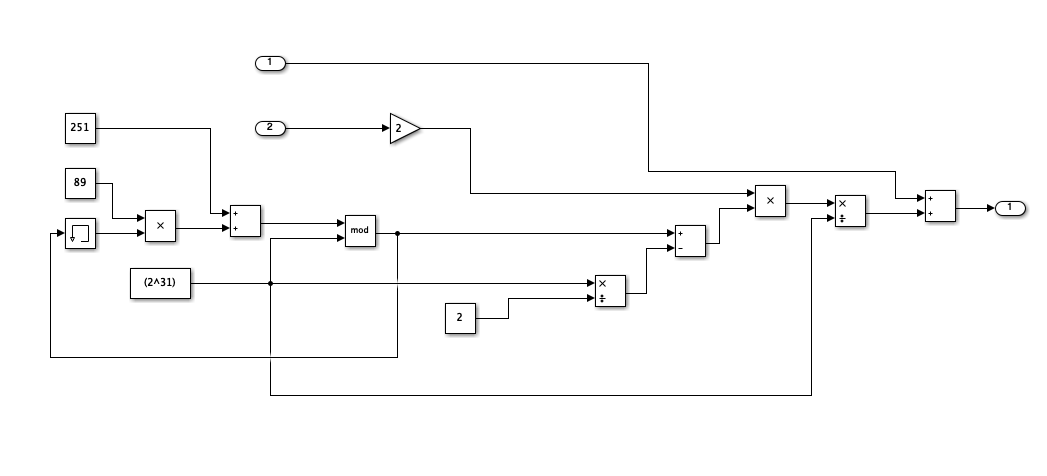
\includegraphics[width=1\linewidth]{../Graphiken/Simulink5}
	\caption{Random Number Generator}
	\label{fig:Simulink5}
\end{figure}